% Auriga theme
% https://github.com/anishathalye/auriga

\documentclass[14pt,aspectratio=169]{beamer}
\usepackage{pgfpages}
\usepackage{fancyvrb}
\usepackage{tikz}
\usepackage{pgfplots}

% Notes
%\ifnotes
%\setbeamertemplate{note page}[plain]
%\setbeameroption{show notes on second screen=right}
%\fi

\usetheme{auriga}
\usecolortheme{auriga}

% Header line
\useoutertheme[subsection=false]{miniframes}

% Footer line
\makeatletter
\def\ps@navigation@titlepage{%
  \setbeamertemplate{footline}{}
  \@nameuse{ps@navigation}
}
\addtobeamertemplate{title page}{\thispagestyle{navigation@titlepage}}{}
\pretocmd{\tableofcontents}{\thispagestyle{navigation@titlepage}}{}{}
\makeatother

% Section Slides
\AtBeginSection[]{
  \begin{frame}
  \vfill
  \centering
  \begin{beamercolorbox}[sep=8pt,center,shadow=true,rounded=true]{title}
    \usebeamerfont{title}\insertsectionhead\par%
  \end{beamercolorbox}
  \vfill
  \end{frame}
}

% adjust caption size
\newcommand\mycaption[1]{{\footnotesize #1}}

% define some colors for a consistent theme across slides
\definecolor{red}{RGB}{181, 23, 0}
\definecolor{blue}{RGB}{0, 118, 186}
\definecolor{gray}{RGB}{146, 146, 146}

% title
\title{Heterogeneity-Robust Spatial Synthetic Controls}
\author{Daniel C Posmik \inst{1}}
\institute[shortinst]{\inst{1} Becker Friedman Institute for Economic Research; University of Chicago \\ E-Mail: posmikdc@uchicago.edu}


% title page
\begin{document}

{
  % rather than use the frame options [noframenumbering,plain], we make the
  % color match, so that the indicated page numbers match PDF page numbers
  \setbeamercolor{page number in head/foot}{fg=background canvas.bg}
  \begin{frame}
    \titlepage
  \end{frame}
}

% body

\begin{frame}{Table of Contents}
  \setbeamertemplate{section in toc}[sections numbered]
  \tableofcontents[hideallsubsections]
\end{frame}
\section{Motivation}
\begin{frame}{Disclaimer}
    \begin{itemize}
        \item{This is a collection of preliminary, high-level ideas.}
        \item{The purpose of this presentation is to receive constructive criticism!}
        \item{My goal is to develop this project into a proper study in graduate school!}
    \end{itemize}
\end{frame}

\begin{frame}{Synthetic Controls \& DiD: A Review}
  \begin{columns}
    \begin{column}{0.58\linewidth}
        \begin{itemize}
            \item{Recover causal effects when no/ few untreated comparison units are available.}
            \vspace{-7pt}
            \item{Construct synthetic control units via pre-treatment/ exogenous characteristics}
            \vspace{-7pt}
            \item{Relies on parallel trends assumption}
            \vspace{-7pt}
            \item{Causal estimator can be recovered in DiD, see Arkhangelsky et al, 2021}
            \vspace{-7pt}
            \item{\textbf{But}: This does not account for treatment effect heterogeneity - No insight into granular treatment responses due to spatial aggregation!}
        \end{itemize}
    \end{column}
    \begin{column}{0.5\linewidth}
        \centering
        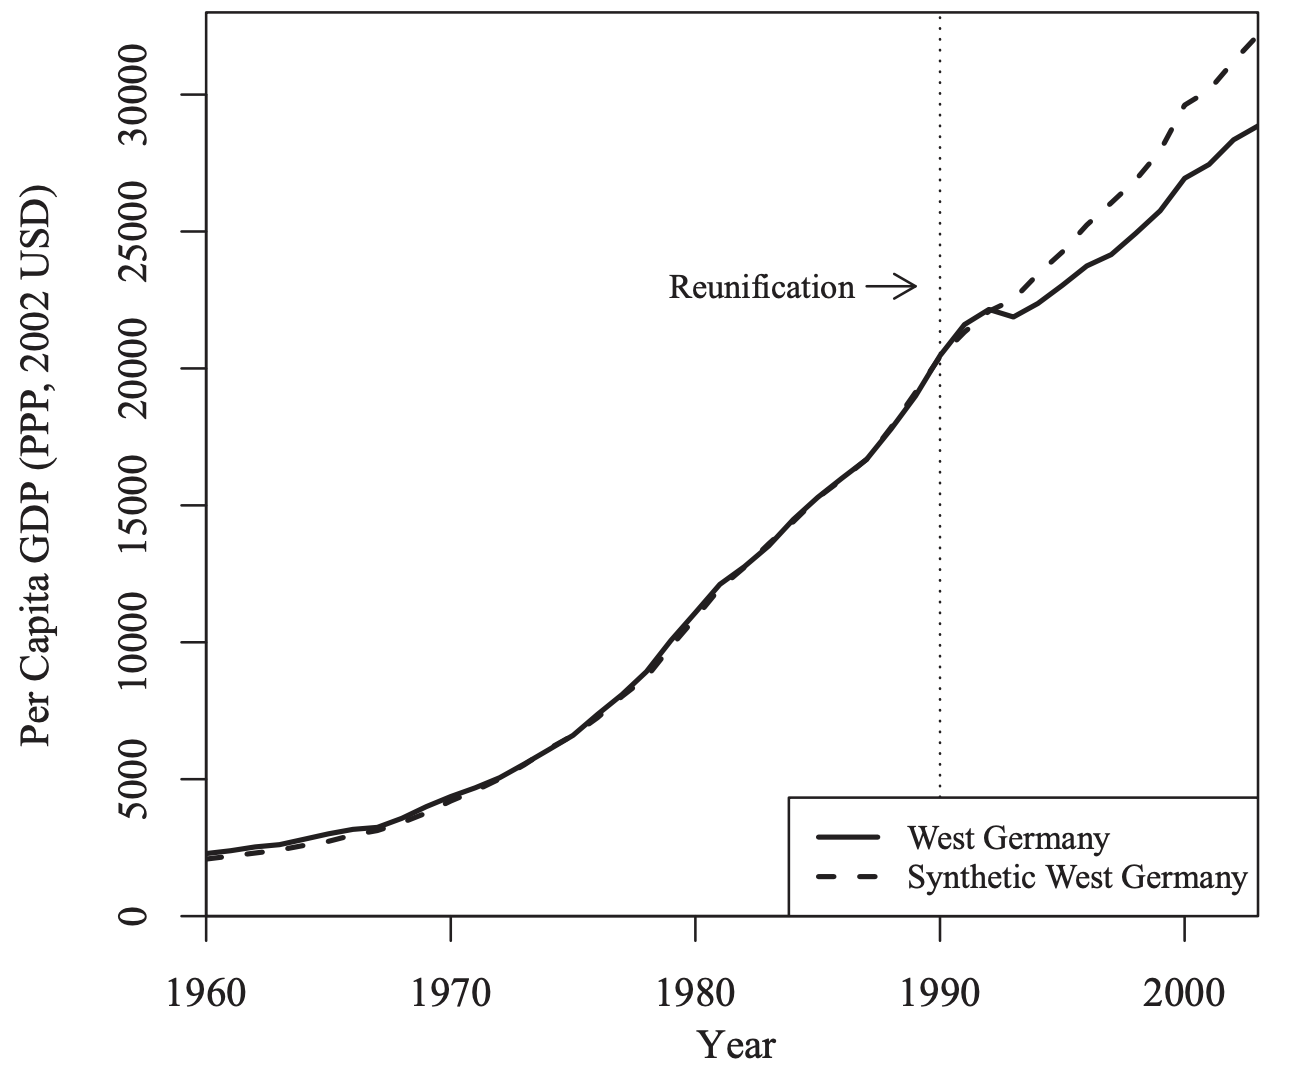
\includegraphics[scale = 0.3]{figures/fig.scmethod.png}\\
        \centering
        \mycaption{\cite{@abadieetal2015}: German Reunification}
    \end{column}
  \end{columns}
\end{frame}

\begin{frame}{Research Goals}

I am interested in measuring the treatment effect $\tau_{it}(x)$ at location $i$ and time $t$. Formally: \\ 
\vspace{3pt}
$\tau_{it}(x) = \E [Y_{it}^{(1)} - Y_{it}^{(0)} | X_{it} = x]$ \\
\vspace{3pt}
where the $Y_{it}^{(1)}$ is the observed treated outcome, $Y_{it}^{(0)}$ denotes the unobserved untreated counterfactual. Let $X_{it}$ denote a set of covariates and $Z_{it}$ the treatment status, where $Z_{it} \in [0,1]^{d}$. \\
\vspace{5pt}
My research goals are:\\
\vspace{3pt}
\begin{itemize}
    \item Proposing a method for counterfactual prediction
    \vspace{-7pt}
    \item Matching comparison units to any treated unit $Y_{it}^{(1)}$
    \vspace{-7pt}
    \item Developing a difference-in-differences estimator
\end{itemize}
\end{frame}
\section{Generating Synthetic Controls}

\begin{frame}{Requirements for the Prediction Algorithm}
    \begin{columns}
    \begin{column}{0.5\linewidth}
    \vspace{5pt}
      \begin{enumerate}
         \item {Model non-linear relationships well}
         \item {Robust to unobservables ("heterogeneity-robust") across spatial and temporal dimensions}
         \item {Suitable for high-dimensional space}
      \end{enumerate}
    \end{column}
    \begin{column}{0.5\linewidth}
      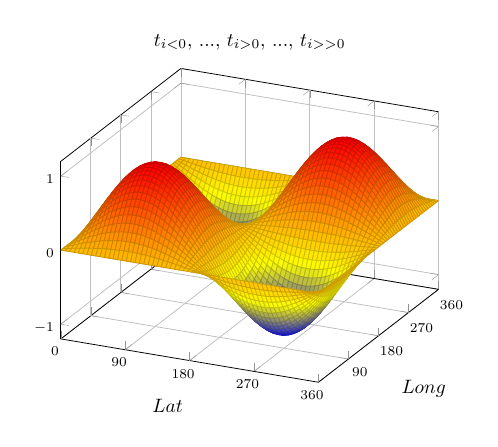
\begin{tikzpicture}[scale=0.70]
      \begin{axis} [
        title = {$t_{i<0}$, ..., $t_{i>0}$, ..., $t_{i>>0}$},
        xtick = {0,90,...,360},
        ytick = {90,180,...,360},
        xlabel = $Lat$, ylabel = $Long$,
        ticklabel style = {font = \scriptsize},
	grid]
        \addplot3 [surf, domain=0:360, samples=60] 
        	{ sin(x)*sin(y) };
        \end{axis}
        \end{tikzpicture}
    \end{column}
  \end{columns}

    \begin{center}
    \vspace{5pt}
    \footnotesize{\textbf{Note}: This problem is currently at the forefront of statistical research. If I had a definitive solution, I would be resting on my laurels right now.}
    \end{center}
\end{frame}

\begin{frame}{Solutions?}

    \begin{table}[htbp]
    \centering
    \begin{tabular}{|p{0.3\linewidth}|p{0.3\linewidth}|p{0.3\linewidth}|}
    \hline
    \textbf{Machine Learning} & \textbf{Non-Parametric} & \textbf{Dimensionality Reduction} \\
    \hline
    Strong predictive performance in non-linear relationships & Robust to violations of functional form assumptions & Absorb temporal dimension into fixed effect. \
    \end{tabular}
    \end{table}
\end{frame}

\begin{frame}{Inspiration from Literature}

\begin{itemize}
    \item \cite{pouliot2022}
      \begin{itemize}
        \item Krig-and-regress method for spatially misaligned data
        \item Introduces Kriging (prediction) method into spatial econometrics
        \item Relevant discussion on interpolation, aggregation, and spatial filtering techniques
      \end{itemize}
    \vspace{-7pt}
    \item \cite{serraburieletal2020}
      \begin{itemize}
        \item Estimate the effects of wildfires on vegetation
        \item An application of spatial synthetic controls, though treatment is discrete and units are static
        \item Use of Nuclear Norm Matrix Completion Method (see, \cite{athey2021}
      \end{itemize}
  \end{itemize}
\end{frame}
\section{Heterogeneous Treatment Effects}

\begin{frame}{A Set of Spatial Treatment Effects}
\begin{itemize}
    \item Assume we have finite spatial grid which is divided in $i∗j$ grids, where $i \in Lat$ and $j \in Long$. 
    \vspace{-7pt}
    \item Then, we can obtain a set of treatment effects $D = \{\delta_{1,1}, \delta_{2,1}, \delta_{1,2}, ..., \delta_{i,j}\}$ by subtracting synthetic untreated outcomes in observed treated outcomes at position $i,j$. 
    \vspace{-7pt}
    \item Commonly, it is assumed that all elements of $D$ are constant over space. This assumption does not hold in spatially heterogeneous settings.
\end{itemize}
\end{frame}

\begin{frame}{Reporting Heterogeneous Treatment Effects}

The set of treatment effects $D$ at time $t_i$ may be spatially heterogeneous:  
\vspace{5pt}

  \begin{columns}
    % Split 1
      \begin{column}{0.45\linewidth}
      \centering
      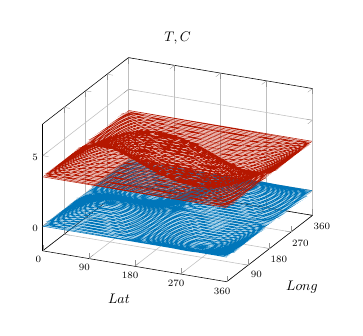
\begin{tikzpicture}[scale=0.50]
      \begin{axis} [
        title = {$T, C$},
        xtick = {0,90,...,360},
        ytick = {90,180,...,360},
        xlabel = $Lat$, ylabel = $Long$,
        ticklabel style = {font = \scriptsize},
	grid]
        \addplot3 [blue, domain=0:360, samples=60] 
        	{ sin(x)*sin(y) };
        \addplot3 [red, domain=0:360, samples=60] 
        	{ sin(0.5*x)*3*sin(y) + 3.5 };
        \end{axis}
        \end{tikzpicture} \\
        \centering{\footnotesize{\textcolor{red}{Treated ($T$)}, \textcolor{blue}{Control ($C$)}}}
    \end{column}
    % Split 2
    \begin{column}{0.45\linewidth}
    \centering
      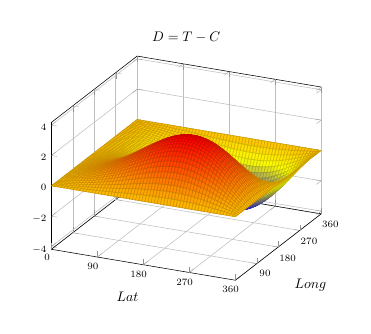
\begin{tikzpicture}[scale=0.50]
      \begin{axis} [
        title = {$D = T - C$},
        xtick = {0,90,...,360},
        ytick = {90,180,...,360},
        xlabel = $Lat$, ylabel = $Long$,
        ticklabel style = {font = \scriptsize},
	grid]
        \addplot3 [surf, domain=0:360, samples=60] 
        	{ sin(0.5*x)*3*sin(y) - sin(x)*sin(y) };
        \end{axis}
        \end{tikzpicture} \\
        \centering{\footnotesize{\textcolor{orange}{Treatment Effects ($D$)}}}
    \end{column}
  \end{columns}
\end{frame}

\begin{frame}{Reporting Heterogeneous Treatment Effects}
\begin{itemize}
    \item How do we report these heterogeneous treatment effects?
    \vspace{-7pt}
\begin{itemize}
    \item Individual Treatment Effect: We report $\delta_{i,j}$ for $\forall i,j$.
    \item Average Treatment Effect: We report $\frac{1}{n}*\sum(\delta_{i,j})$ $\forall i,j$. 
\end{itemize}
    \vspace{-7pt}
    \item The options are unrealistic and uninformative, respectively. Therefore, can we find a good middle ground?
\end{itemize}

\begin{center}
    Formally: We are looking to report the average of k subsets of $D$, where $1 < k < n$ in a plane with $n$ grids. 
\end{center}
\end{frame}

\begin{frame}{The Clustering Problem}
    Rather than pre-define the reporting veracity (e.g., zip code), a clustering approach may allow the data to tell the whole story. 
    \vspace{5pt}

  \begin{columns}
    % Split 1
      \begin{column}{0.6\linewidth}
      \begin{itemize}
          \item How do we find the optimal k?
          \vspace{-7pt}
          \item Problem: As $n$ increases, the error function monotonically decreases
          \vspace{-7pt}
          \item Formally: $\nexists k$ s.t. $argmin_{k}$(Error), outside of $k = n$. 
      \end{itemize}
    \end{column}
    % Split 2
    \begin{column}{0.45\linewidth}
        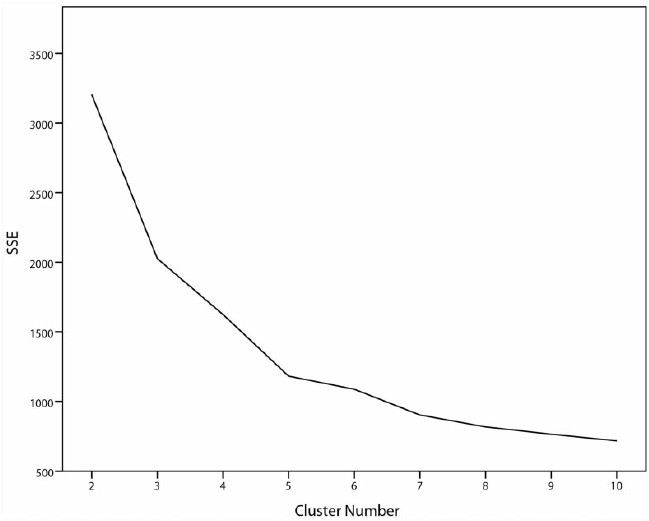
\includegraphics[scale = 0.21]{figures/sse_cluster-n_tradeoff.jpg}\\
        \mycaption{Trade-Off: SSE vs. Cluster #}
    \end{column}
  \end{columns}
\end{frame}

\begin{frame}{The Clustering Problem}

\begin{itemize}
    \item How do we report these heterogeneous treatment effects?
    \vspace{-7pt}
\begin{itemize}
    \item Individual Treatment Effect: We report $\delta_{i,j}$ for $\forall i,j$.
    \item Average Treatment Effect: We report $\frac{1}{n}*\sum(\delta_{i,j})$ $\forall i,j$. 
\end{itemize}
    \vspace{-7pt}
    \item The options are unrealistic and uninformative, respectively. Therefore, can we find a good middle ground?
\end{itemize}

\begin{center}
    Formally: We are looking to report the average of k subsets of $D$, where $1 < k < n$ in a plane with $n$ grids. 
\end{center}
\end{frame}

\begin{frame}{A Solution?}
Rather than pre-define the reporting veracity (e.g., zip code), a clustering approach may allow the data to tell the whole story. 
\vspace{5pt}

  \begin{columns}
    % Split 1
      \begin{column}{0.6\linewidth}
      \begin{itemize}
          \item Methods to find $k$: Elbow, Silhouette, etc.
          \vspace{-7pt}
          \item Problem: Curse of dimensionality!
          \vspace{-7pt}
          \item Uncertain: Is time really that important in short time horizons? 
      \end{itemize}
    \end{column}
    % Split 2
    \begin{column}{0.45\linewidth}
        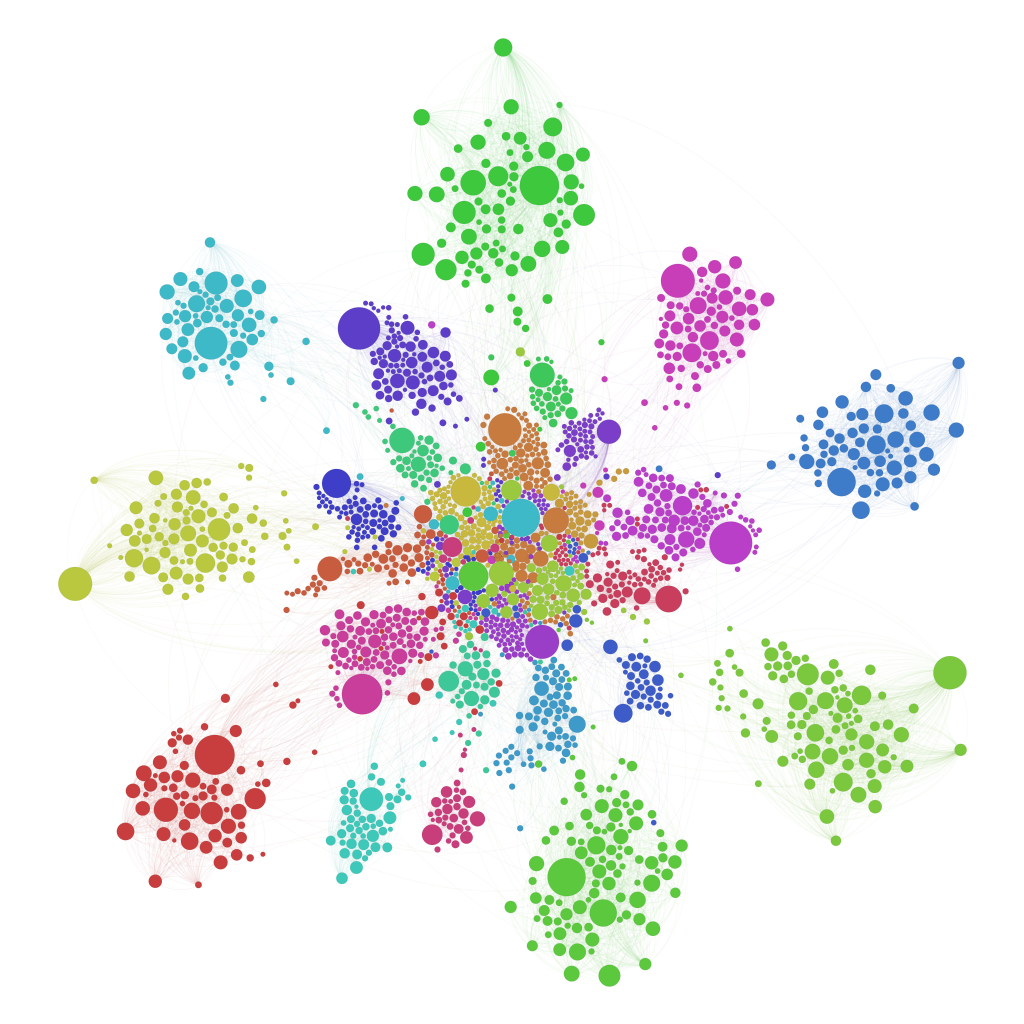
\includegraphics[scale = 0.12]{figures/high-dim_clustering.jpg}\\
        \mycaption{High-dimensional Clustering}
    \end{column}
  \end{columns}
\end{frame}
\section{Heatwave Application}

\begin{frame}{Motivation}

  \begin{columns}
    \begin{column}{0.6\linewidth}
      \begin{itemize}
        \item Measuring the effect of climate disasters
            \begin{itemize}
            \item Experimental approaches - if not unethical - are nearly impossible
            \item Researchers are stuck with observational data
            \item Recovering robust causal effects is critical policy input
            \end{itemize}
      \end{itemize}
    \end{column}
    \begin{column}{0.4\linewidth}
      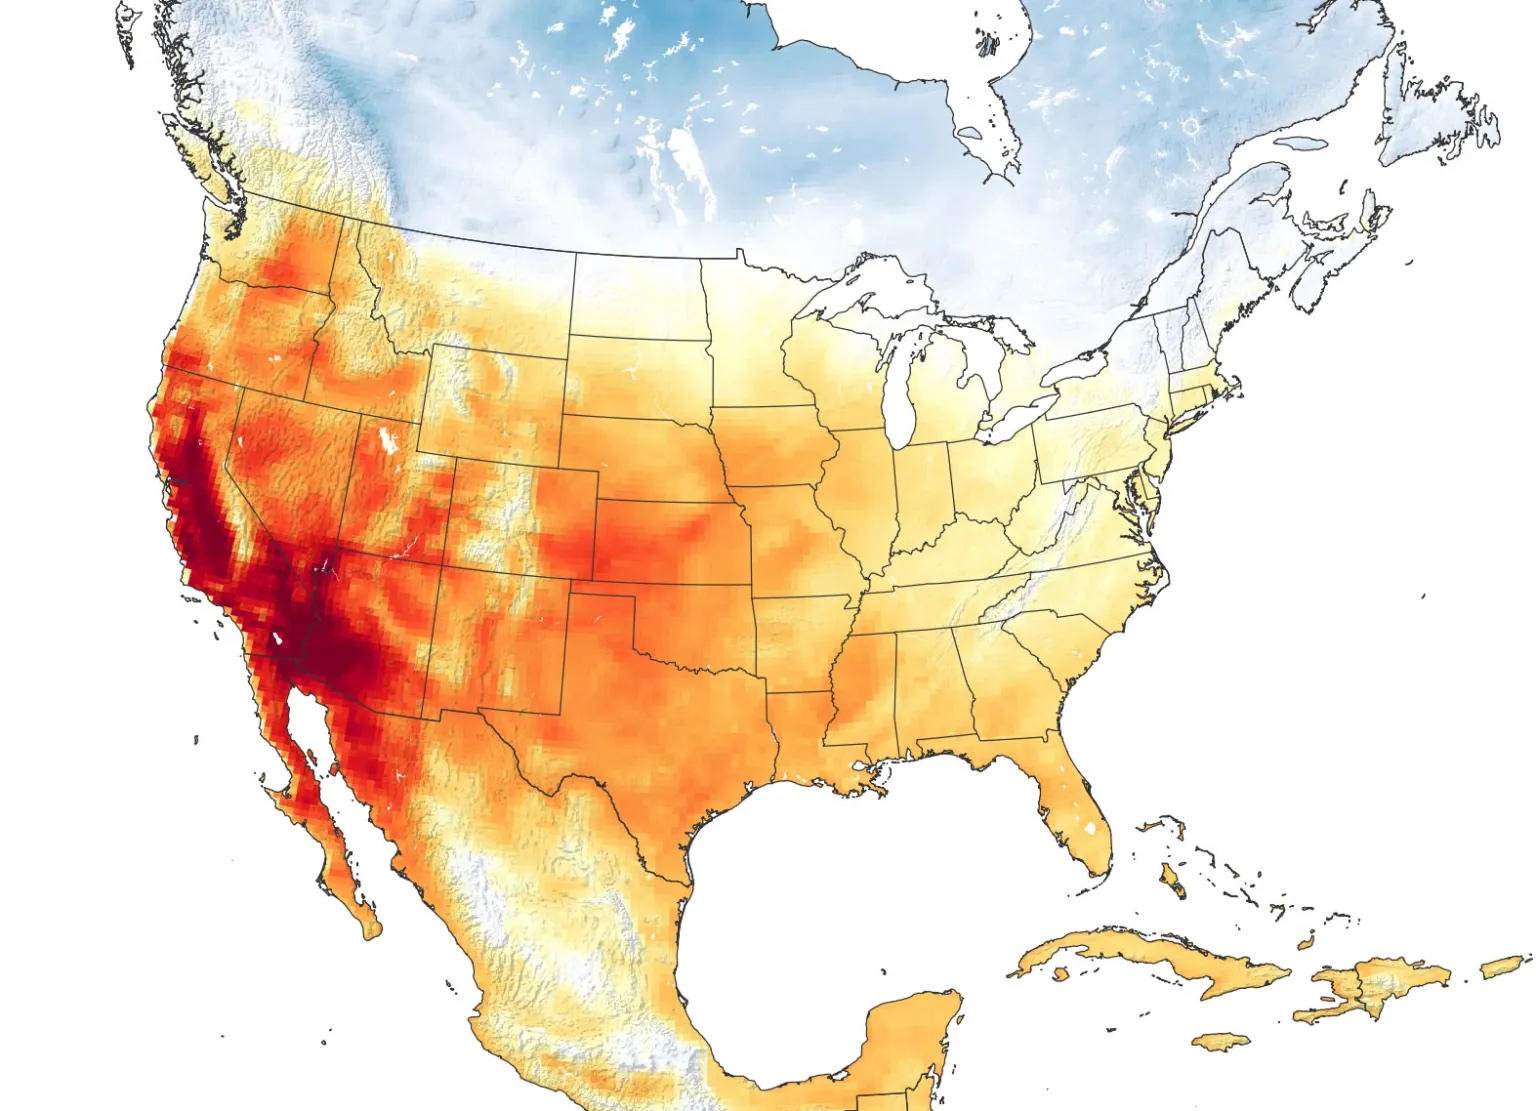
\includegraphics[scale=0.1]{figures/california-heatwave-2020-nasa-eo.jpeg}
      \caption{}
    \end{column}
  \end{columns}

\vspace{7pt}
\begin{center}
    \textbf{My Research Question: What is the effect of heat waves on hospitalization rates?}
\end{center}

  \note{
    This slide has notes too.
  }

\end{frame}

\begin{frame}{U.S. Cell Phone Ping Data}
Access to cell phone ping data: Unique opportunity to analyze spatial settings where units are not bound to spatial location.
\vspace{5pt}
\begin{columns}
    % Split 1
    \begin{column}{0.65\linewidth}
    \begin{itemize}
    \item Consider a densely populated area:
    \vspace{-7pt}
    \item Idea 1: Measure whether individuals visit hospitals via cell phone pings (Problem: Ping Irregularity)
    \vspace{-7pt}
    \item Idea 2: Measure the \textit{dispersion effect} of heat waves
    \end{itemize}
    \end{column}
    % Split 2
     \begin{column}{0.4\linewidth}
      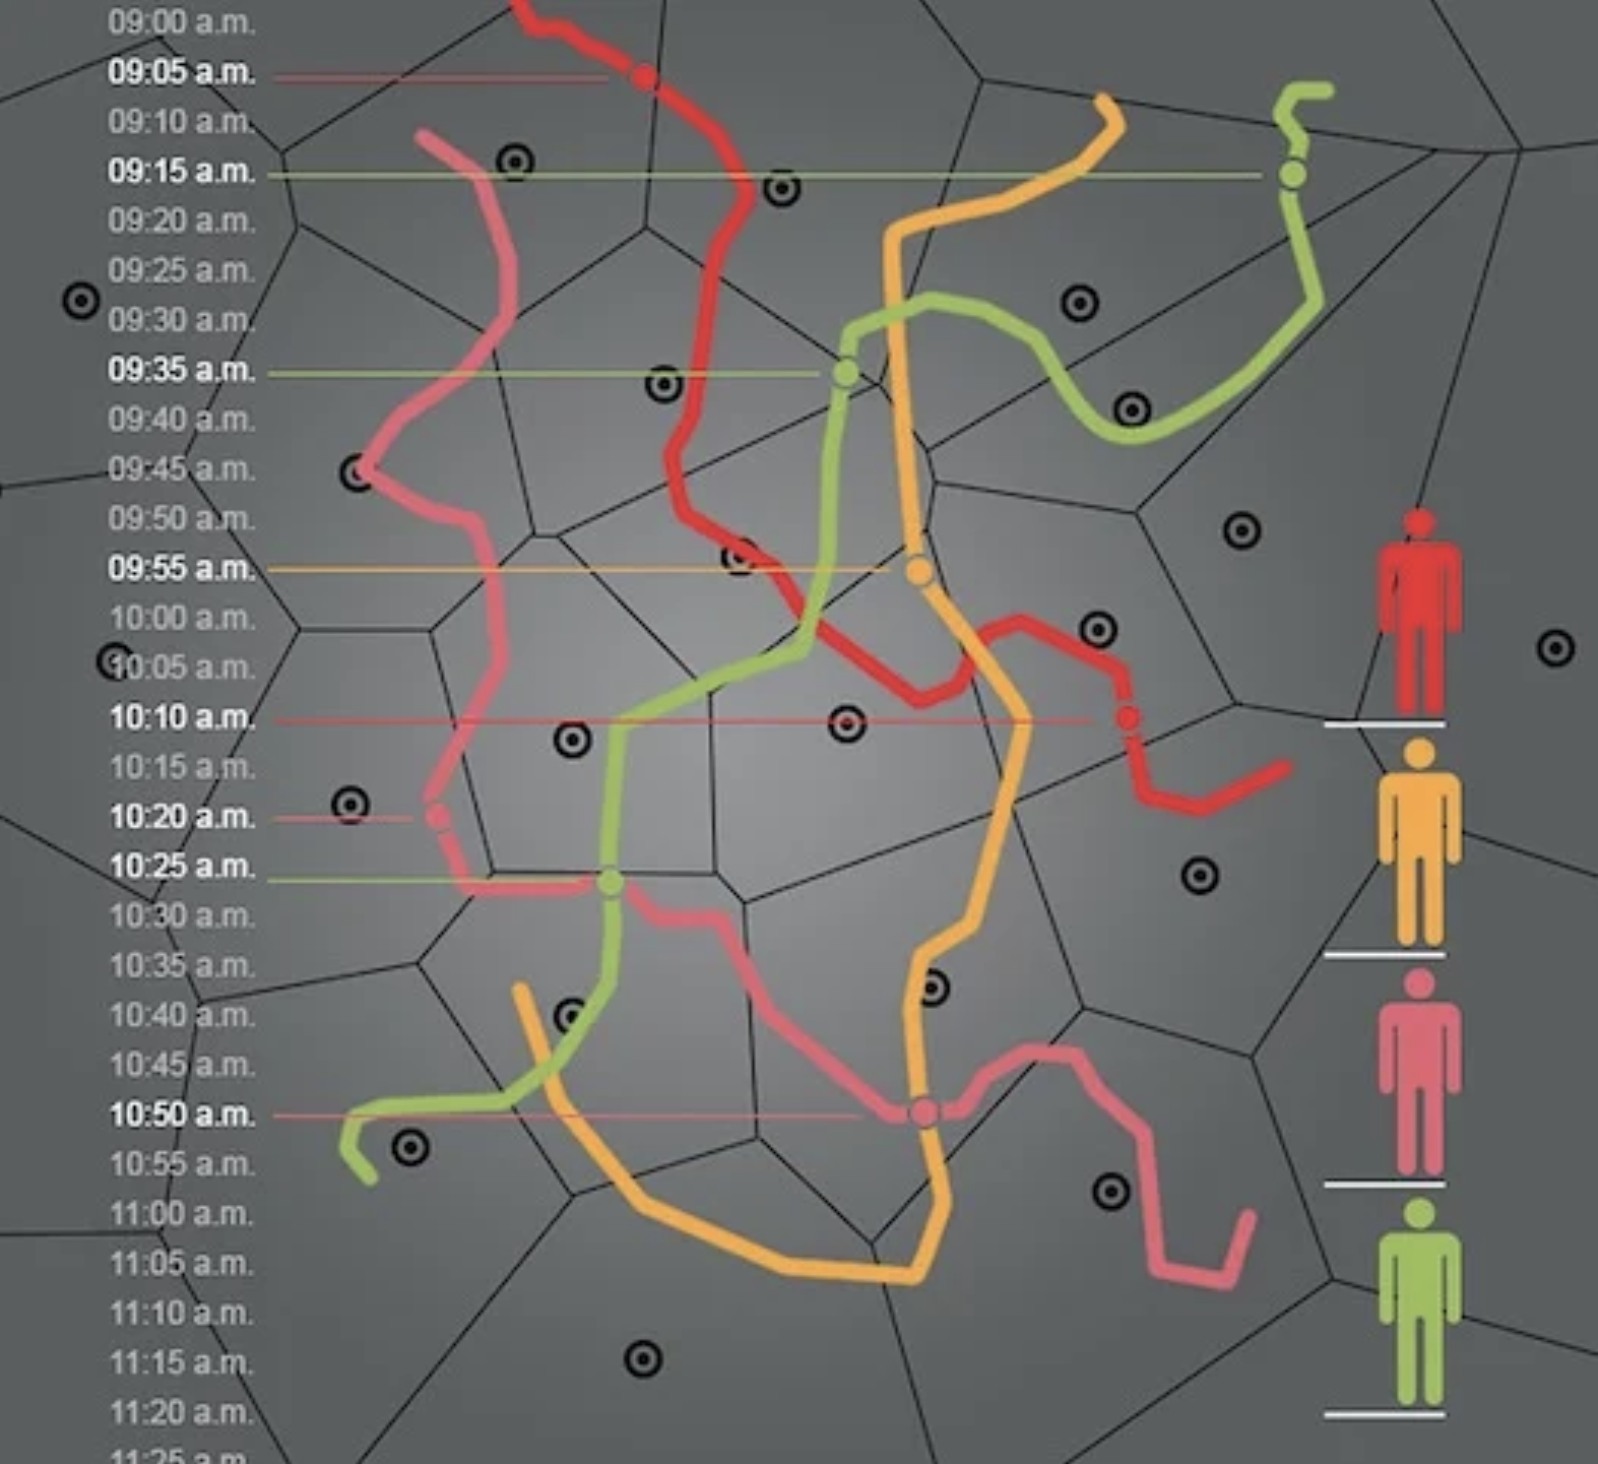
\includegraphics[scale=0.16]{figures/cell_ping.png}
      \caption{}
    \end{column}
\end{columns}
\end{frame}

\begin{frame}{Brainstorming}
- Think about mapping hospitals etc. 
- But also public facilities that are AC controlled??? These could be identified with the help of and conversations with community members and stewards
- Insight maybe: High-income - ppl just hunker down in their AC controlled places; low-income: Do people try to "escape"/ "flee" the heat to other places???
- classify/ define the concept of a "HEAT SHELTER" in addition to hospitals
- Define the median location of an individual as their home; also look into work location?
\end{frame}
\section{Conclusion and Discussion}

\begin{frame}{Further Extensions}
\begin{itemize}
    \item Continuous treatment (consider \cite{callawayetal2021})
    \item Recent advances in spatial treatments (see, M. Pollmann)
    \item Digging into high-dimensional prediction and clustering
\end{itemize}
\end{frame}

% Appendix----------------------------------------------------------------
\appendix

% References--------------------------------------------------------------
\begin{frame}[allowframebreaks]{References}
  \bibliography{main.bib}
  \bibliographystyle{apalike}
\end{frame}

\end{document}
